\chapter{Penrose Diagrams and the Formation of a Real Black Hole}

These notes follow the lecture in the order in which the argument is actually built. We begin with the near-horizon Kruskal picture, step back to compactify flat spacetime, return to the black hole in Penrose form, and then use the same causal technology to describe the formation of a real black hole by an infalling shell of radiation. The lecture is by Leonard Susskind, and where the blackboard itself carries mathematical content we keep the original board evidence alongside cleaner reconstructions; the preserved stills used here were curated through LazyingArt LLC and Video2Book.

\section{Near the Horizon: Kruskal Recap and the Four Quadrants}

We begin exactly where the previous lecture left off. Very near the Schwarzschild horizon, the geometry looks locally like flat space. The horizon itself behaves like a hyperbolic polar-coordinate locus, very much in the same spirit as accelerated coordinates in ordinary Minkowski spacetime. In this local description we adopt one simple kinematic rule and never let go of it: radial light rays are drawn at \(45^\circ\), and any timelike worldline must remain steeper than those null lines.

The lecture uses this picture to distinguish two different kinds of motion. First, there are freely falling observers, for whom the local geometry near the horizon looks approximately flat. Second, there are observers held at fixed radius outside the hole. Relative to the infalling coordinates, those stationary observers trace accelerated curves. The closer one hovers to the horizon, the larger the required acceleration. That is why the family of exterior curves bends more sharply as it approaches the horizon.

\begin{figure}[htbp]
\centering

\includegraphics[width=0.72\textwidth]{lecture_08_figure_02.png}
\caption{Board sketch of the four-region near-horizon geometry. The red curves in the exterior record a family of hovering worldlines at fixed radius.}
\end{figure}

\begin{figure}[htbp]
\centering
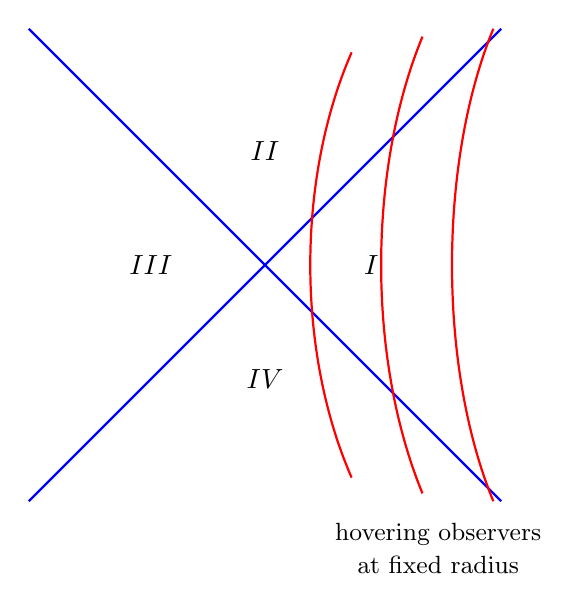
\begin{tikzpicture}[scale=1.0]
\draw[thick,blue] (-3,3) -- (3,-3);
\draw[thick,blue] (-3,-3) -- (3,3);

\draw[red,thick] (1.1,-2.7) .. controls (0.4,-1.1) and (0.4,1.1) .. (1.1,2.7);
\draw[red,thick] (2.0,-2.9) .. controls (1.3,-1.2) and (1.3,1.2) .. (2.0,2.9);
\draw[red,thick] (2.9,-3.0) .. controls (2.2,-1.3) and (2.2,1.3) .. (2.9,3.0);

\node at (1.35,0.0) {$I$};
\node at (0.0,1.45) {$II$};
\node at (-1.45,0.0) {$III$};
\node at (0.0,-1.45) {$IV$};

\node[align=center] at (2.2,-3.6) {\small hovering observers\\\small at fixed radius};
\end{tikzpicture}
\caption{Clean redraw of the Kruskal-style causal structure used in the recap. Region \(I\) is the exterior, region \(II\) the inescapable interior, and regions \(III\) and \(IV\) belong to the formal extension that will later be discarded for a real collapsing black hole.}
\end{figure}

The lecture then sharpens the physical reading. Region \(I\) is the outside of the black hole. Region \(II\) is the interior, and once one is there the causal verdict is already fixed: every future-directed timelike trajectory ends on the singularity. The transcript is garbled in part of this discussion, but the mathematical point is secure. To escape from region \(II\) into either exterior region would require a trajectory shallower than \(45^\circ\) somewhere, and therefore superluminal motion.

This is already the first warning signal of the chapter. The full Kruskal picture is elegant, but not every part of it belongs to a real black hole formed in the world.

\section{From Infinite Spacetime to a Finite Board}

The next move is pedagogically essential. If we want to decide what part of the Kruskal story is physically meaningful, we need a way to draw an entire spacetime on a finite blackboard without destroying the role of light cones. That is what motivates Penrose diagrams. The lecturer does not introduce them abstractly; he begins with ordinary flat spacetime and teaches the compactification in the simplest possible arena.

Because the spacetimes under discussion are spherically symmetric, we suppress the angular directions and keep only time and the radial coordinate. We therefore use coordinates \(T\) and \(R\), with
\[
R\ge 0,
\]
since negative radial distance has no polar-coordinate meaning. Throughout we set
\[
c=1.
\]
With that choice, radial null motion is drawn at \(45^\circ\).

There is one small subtlety. In the reduced radial picture, a light ray aimed exactly at the origin appears to bounce from the line \(R=0\). The lecture is careful about this: nothing physical is reflecting from a wall. In the full spherically symmetric geometry the ray simply passes through the origin and re-emerges on the other side. The apparent bounce is only a consequence of using the radial coordinate \(R\ge 0\).

\begin{figure}[htbp]
\centering

\includegraphics[width=0.82\textwidth]{lecture_08_figure_03.png}
\caption{Board derivation of the null-coordinate combinations \(T+R=T^+\) and \(T-R=T^-\), together with the associated \(T\)-\(R\) sketch.}
\end{figure}

The crucial step is to introduce null coordinates:
\begin{align}
T^+ &= T+R, \\
T^- &= T-R.
\end{align}
These are adapted to radial light rays. An ingoing radial null ray has \(T^+=\text{const}\), while an outgoing radial null ray has \(T^-=\text{const}\).

\paragraph{Worked derivation.}
The line \(R=0\) becomes particularly simple in these coordinates. Indeed,
\begin{align}
R=0
&\iff T+R=T-R \\
&\iff T^+=T^-.
\end{align}
So the entire timelike boundary \(R=0\) is described by the single relation
\begin{equation}
R=0 \iff T^+=T^-.
\end{equation}

Now we compactify. We introduce two new null coordinates \(U^\pm\), each obtained from the corresponding \(T^\pm\) by the same bounded monotone function \(F\):
\begin{align}
U^+ &= F(T^+), &
U^- &= F(T^-),
\end{align}
with
\begin{equation}
F(+\infty)=1,
\qquad
F(-\infty)=-1.
\end{equation}
The convenient lecture choice is
\begin{equation}
F(x)=\tanh x,
\end{equation}
so that
\begin{equation}
U^+ = \tanh(T^+),
\qquad
U^- = \tanh(T^-).
\end{equation}

This preserves the null structure for a very simple reason. If an ingoing radial light ray has \(T^+=\text{const}\), then
\[
U^+=F(T^+)=\text{const},
\]
and similarly if an outgoing radial light ray has \(T^-=\text{const}\), then \(U^-=\text{const}\). In other words, the compactification separately reparametrizes the two null directions, and therefore radial light rays remain \(45^\circ\) lines.

The boundary \(R=0\) is carried along with no difficulty:
\[
T^+=T^- \Longrightarrow U^+=U^-.
\]
Thus the origin line remains the line \(U^+=U^-\) in the compactified picture.

\begin{figure}[htbp]
\centering
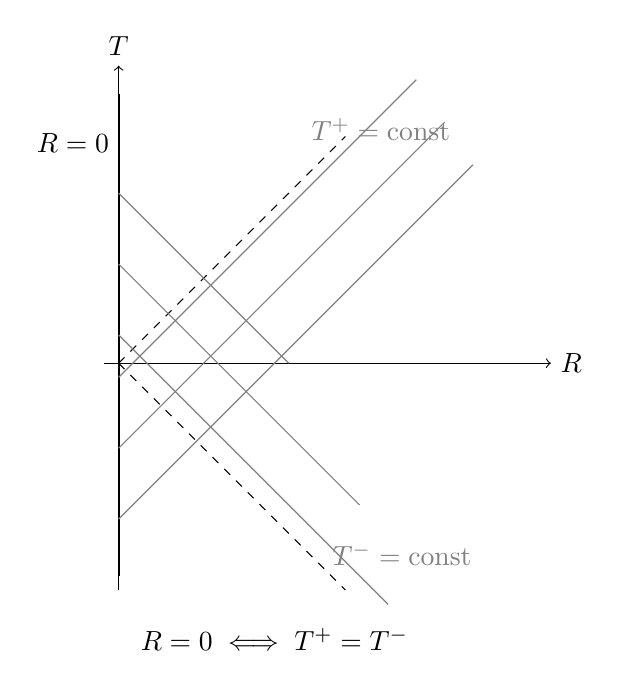
\begin{tikzpicture}[scale=0.9]
\draw[->] (-0.2,0) -- (6.1,0) node[right] {$R$};
\draw[->] (0,-3.2) -- (0,4.2) node[above] {$T$};

\draw[thick] (0,-3.0) -- (0,3.8);
\node[left] at (0,3.1) {$R=0$};

\draw[dashed] (0,0) -- (3.2,3.2);
\draw[dashed] (0,0) -- (3.2,-3.2);

\draw[gray] (0,2.4) -- (2.4,0);
\draw[gray] (0,1.4) -- (3.4,-2.0);
\draw[gray] (0,0.4) -- (3.8,-3.4);

\draw[gray] (0,-2.2) -- (5.0,2.8);
\draw[gray] (0,-1.2) -- (4.6,3.4);
\draw[gray] (0,-0.2) -- (4.2,4.0);

\node[gray] at (3.7,3.3) {$T^+=\mathrm{const}$};
\node[gray] at (4.0,-2.7) {$T^-=\mathrm{const}$};

\node at (2.2,-3.9) {$R=0 \iff T^+=T^-$};
\end{tikzpicture}
\caption{A clean \(T\)-\(R\) redraw. The two null families are the level sets of \(T^+\) and \(T^-\), and the line \(R=0\) is equivalently \(T^+=T^-\).}
\end{figure}

Once the geometry has been squeezed into a finite region, we can read off the compactified boundary. Spatial infinity collapses to a single point \(i^0\). Future and past timelike infinities are \(i^+\) and \(i^-\). The incoming and outgoing null boundaries are \(\mathscr I^-\) and \(\mathscr I^+\), the places where radial light rays begin and end.

\begin{figure}[htbp]
\centering
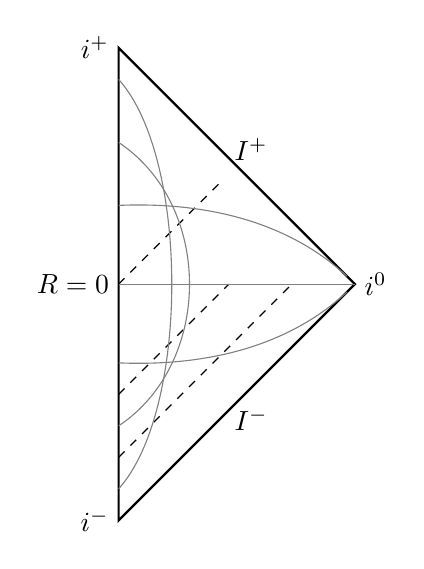
\begin{tikzpicture}[scale=1.0]
\draw[thick] (0,-3) -- (0,3) -- (3,0) -- cycle;

\node[left] at (0,3) {$i^+$};
\node[left] at (0,-3) {$i^-$};
\node[right] at (3,0) {$i^0$};
\node[left] at (0,0) {$R=0$};
\node[above right] at (1.35,1.45) {$\mathscr I^+$};
\node[below right] at (1.35,-1.45) {$\mathscr I^-$};

\draw[dashed] (0,-2.2) -- (2.2,0.0);
\draw[dashed] (0,-1.4) -- (1.4,0.0);
\draw[dashed] (0,0.0) -- (1.3,1.3);

\draw[gray] (0,0) -- (3,0);
\draw[gray] (0,1.0) .. controls (1.2,1.05) and (2.2,0.75) .. (2.9,0.1);
\draw[gray] (0,-1.0) .. controls (1.2,-1.05) and (2.2,-0.75) .. (2.9,-0.1);

\draw[gray] (0,-2.6) .. controls (0.9,-1.6) and (0.9,1.6) .. (0,2.6);
\draw[gray] (0,-1.8) .. controls (1.2,-1.0) and (1.2,1.0) .. (0,1.8);
\end{tikzpicture}
\caption{Transcript-backed reconstruction of the Penrose diagram for radially reduced flat spacetime. Constant-time curves accumulate near the null boundary, while constant-radius curves run upward toward timelike infinity.}
\end{figure}

The moral of the construction is already clear. We are free to squeeze, stretch, and distort the drawing, but we insist on preserving one piece of structure: radial light rays remain null lines at \(45^\circ\). This is what compactification is for.

\section{The Compactified Schwarzschild Geometry}

Now we return to the black hole. The lecture applies exactly the same compactification logic to the Kruskal geometry. One again introduces null combinations and squeezes the infinite coordinate ranges down to a finite figure. The result is the Penrose diagram of the Schwarzschild black hole.

The lecturer describes the compactified picture as a finite causal figure in which the exterior hovering worldlines remain outside the horizon, the interior region is inescapable, and the singularity becomes a finite future boundary rather than some point at infinity. This last point matters. The singularity is not infinitely far away in the experience of an infalling observer. The proper time from horizon crossing to the singularity is finite.

The horizon is still identified by the Schwarzschild condition
\begin{equation}
1-\frac{2MG}{r}=0
\qquad \Longleftrightarrow \qquad
r=2MG.
\end{equation}
This is the same distinguished radius at which the familiar Schwarzschild factor changes sign.

\begin{figure}[htbp]
\centering

\includegraphics[width=0.72\textwidth]{lecture_08_figure_04.png}
\caption{Board sketch contrasting the formal extended picture with the physically relevant black-hole region. The red label \emph{singularity} is explicit on the board.}
\end{figure}

\begin{figure}[htbp]
\centering
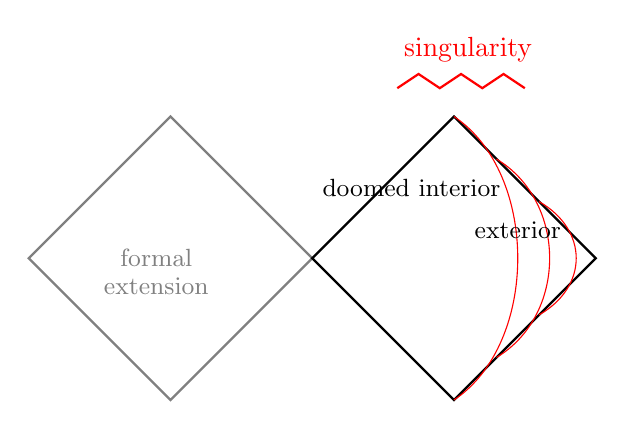
\begin{tikzpicture}[scale=0.9]
\draw[gray,thick] (-4,0) -- (-2,2) -- (0,0) -- (-2,-2) -- cycle;
\draw[thick] (0,0) -- (2,2) -- (4,0) -- (2,-2) -- cycle;

\draw[red,thick] (1.2,2.4) -- (1.5,2.6) -- (1.8,2.4) -- (2.1,2.6) -- (2.4,2.4) -- (2.7,2.6) -- (3.0,2.4);
\node[red] at (2.2,2.95) {singularity};

\draw[red] (2.0,-2.0) .. controls (3.2,-1.2) and (3.2,1.2) .. (2.0,2.0);
\draw[red] (2.6,-1.4) .. controls (3.6,-0.8) and (3.6,0.8) .. (2.6,1.4);
\draw[red] (3.2,-0.8) .. controls (3.9,-0.4) and (3.9,0.4) .. (3.2,0.8);

\node at (2.9,0.4) {\small exterior};
\node at (1.4,1.0) {\small doomed interior};
\node[gray] at (-2.2,0.0) {\small formal};
\node[gray] at (-2.2,-0.4) {\small extension};
\end{tikzpicture}
\caption{A conservative redraw of the causal picture emphasized in the lecture: the exterior region, the doomed interior, the future singularity, and the surviving contrast with the extra formal parts of the extended solution.}
\end{figure}

In the exterior region one can remain outside or fall inward. In the interior region one cannot escape. Any future-directed timelike worldline there ends on the singularity. The Penrose diagram makes this immediate: the light cones tip in such a way that every allowed future motion points toward the singularity.

\subsection{Question \& Answer}

\paragraph{Question.} What are quadrants \(III\) and \(IV\), and do they belong to a real black hole?

\paragraph{Answer.} As parts of the maximally extended Kruskal solution, they are legitimate pieces of the formal analytic extension. One may read them as an additional exterior region together with its time-reversed partner. But this lecture is driving toward a different point: a real black hole formed by collapse does not contain those regions. The physical story preserves the causal lesson of the exterior and interior of the black hole, but not the whole eternal extension. The left-hand side of the full Kruskal diagram is mathematically seductive and physically misleading.

\section{Spatial Slices, Two-Spheres, and the Einstein--Rosen Bridge}

At this stage the lecture freezes time and asks what a spacelike slice of the extended geometry looks like as \emph{space}. This is where the familiar wormhole image enters. But before the picture can be read correctly, one must remember what a point in the reduced diagram means.

Because we have suppressed the angular coordinates, each point of the radial diagram actually stands for a two-sphere. At Schwarzschild radius \(r\), that sphere has area
\begin{equation}
A = 4\pi r^2.
\end{equation}
So a spacelike slice through the extended diagram is not a one-dimensional line in the full geometry. It is a family of two-spheres whose size changes as one moves along the slice.

Far away, \(r\) is large and the corresponding sphere is large. As one moves inward, the sphere shrinks, reaching a minimum size at the horizon,
\begin{equation}
r_{\min}=2MG.
\end{equation}
If one continues along the formal extension, the sphere expands again toward another asymptotic exterior region. This is the Einstein--Rosen bridge picture.

\begin{figure}[htbp]
\centering

\includegraphics[width=0.72\textwidth]{lecture_08_figure_05.png}
\caption{Board sketch of the bridge geometry. The visible Schwarzschild factor fragment at upper left ties the picture to the distinguished radius \(r=2MG\).}
\end{figure}

The lecture uses the visible Schwarzschild factor only as a reminder that the same distinguished combination remains in the background:
\begin{equation}
1-\frac{2MG}{r}.
\end{equation}
The throat sits where this factor vanishes, namely at \(r=2MG\).

\begin{figure}[htbp]
\centering
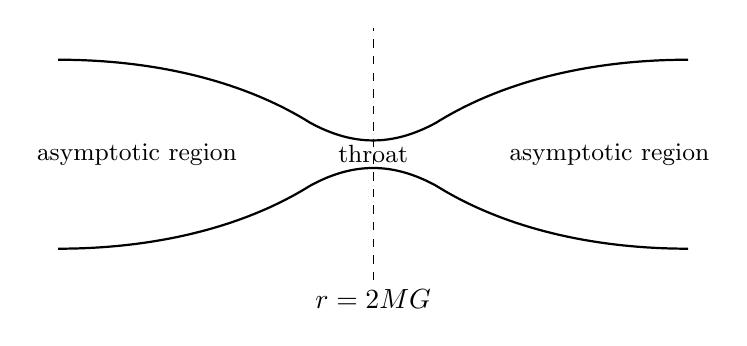
\begin{tikzpicture}[scale=1.0]
\draw[thick] (-4,1.2)
.. controls (-2.7,1.2) and (-1.6,0.9) .. (-0.8,0.4)
.. controls (-0.25,0.1) and (0.25,0.1) .. (0.8,0.4)
.. controls (1.6,0.9) and (2.7,1.2) .. (4,1.2);

\draw[thick] (-4,-1.2)
.. controls (-2.7,-1.2) and (-1.6,-0.9) .. (-0.8,-0.4)
.. controls (-0.25,-0.1) and (0.25,-0.1) .. (0.8,-0.4)
.. controls (1.6,-0.9) and (2.7,-1.2) .. (4,-1.2);

\draw[dashed] (0,-1.6) -- (0,1.6);
\node[below] at (0,-1.6) {$r=2MG$};
\node at (0,0) {\small throat};
\node at (-3.0,0) {\small asymptotic region};
\node at (3.0,0) {\small asymptotic region};
\end{tikzpicture}
\caption{Schematic spatial slice through the extended Schwarzschild geometry. This is a cautious reconstruction of the lecture's bridge picture, not a literal embedding calculation.}
\end{figure}

The important point, however, is not the shape of the bridge but its causal status. One might be tempted to think that the two asymptotic sides are connected by a traversable passage. The Penrose diagram rules this out immediately. To move from one exterior region to the other, a worldline would have to become shallower than a \(45^\circ\) null line somewhere. That would mean faster-than-light motion. The Einstein--Rosen bridge is therefore non-traversable. It is a bridge only as a spacelike slice of the formal extended geometry, not as a route by which a physical observer can travel.

\section{Building a Real Black Hole from an Infalling Null Shell}

Having stripped the eternal diagram of its false promise, the lecture turns to the real physical problem: how to form a black hole from collapse. The model is chosen for simplicity. We do not throw in a star with complicated internal structure. We imagine instead a thin spherical shell of incoming radiation, a shell of light, collapsing inward at the speed of light.

The second ingredient is the shell theorem in its general-relativistic form.

\begin{remark}
For the spherically symmetric shell used in this lecture, the interior region is flat spacetime, while the exterior region is Schwarzschild. This is the operational shell theorem, or Birkhoff-type statement, used by the lecture. It is not proved here.
\end{remark}

This immediately tells us how to construct the spacetime. The shell itself is a null surface, so in the Penrose diagram it must be drawn as a \(45^\circ\) ingoing line. On one side of that line the geometry is flat. On the other side it is Schwarzschild.

It is useful to write the rule in the barest possible form:
\begin{equation}
\text{inside shell} = \text{flat spacetime},
\qquad
\text{outside shell} = \text{Schwarzschild geometry}.
\end{equation}

The gluing prescription is then straightforward:

\begin{enumerate}
\item Draw the flat Penrose diagram and keep only the region interior to the incoming shell.
\item Draw the Schwarzschild Penrose diagram and keep only the region exterior to that same shell.
\item Throw away the unphysical pieces.
\item Glue the surviving parts together along the shell trajectory.
\end{enumerate}

That glued spacetime is the Penrose diagram of a black hole formed by collapse.

\begin{figure}[htbp]
\centering
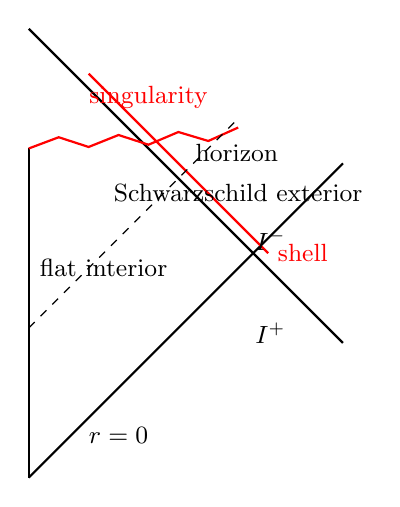
\begin{tikzpicture}[scale=0.95]
\draw[thick] (0,-3.0) -- (0,1.4);
\draw[thick] (0,3.0) -- (4.2,-1.2);
\draw[thick] (0,-3.0) -- (4.2,1.2);

\draw[red,thick] (0.0,1.4) -- (0.4,1.55) -- (0.8,1.42) -- (1.2,1.58) -- (1.6,1.45) -- (2.0,1.62) -- (2.4,1.50) -- (2.8,1.68);
\node[red,above] at (1.6,1.8) {\small singularity};

\draw[thick,red] (3.2,0.0) -- (0.8,2.4);
\node[right,red] at (3.2,0.0) {\small shell};

\draw[dashed] (0,-1.0) -- (2.8,1.8);
\node[above right] at (2.1,1.1) {\small horizon};

\node at (1.0,-0.2) {\small flat interior};
\node at (2.8,0.8) {\small Schwarzschild exterior};

\node[below] at (1.2,-2.2) {\small \(r=0\)};
\node[below right] at (2.9,-0.8) {\small \(\mathscr I^+\)};
\node[above right] at (2.9,-0.1) {\small \(\mathscr I^-\)};
\end{tikzpicture}
\caption{Transcript-backed reconstruction of the collapse geometry. The shell is an ingoing null line; flat spacetime is kept on its interior side, and Schwarzschild geometry on its exterior side.}
\end{figure}

The shell itself feels nothing special merely because it is null; it continues inward and eventually strikes the singularity. The causal meaning of the geometry is carried not by metric sizes on the page, but by which future-directed null and timelike curves can still escape.

\section{The Horizon Before the Shell Arrives}

Now comes the conceptual climax. Once the collapse spacetime has been assembled, the natural question is: where is the horizon? Or, more sharply, where is the true point of no return?

\begin{definition}
The event horizon is the boundary between those events that can still send a future-directed causal signal to \(\mathscr I^+\) and those that cannot.
\end{definition}

The lecture locates it diagrammatically. Start at the corner where the singularity meets future null infinity, and trace a \(45^\circ\) null line backward into the diagram. That backward-traced null line is the event horizon.

\begin{figure}[htbp]
\centering
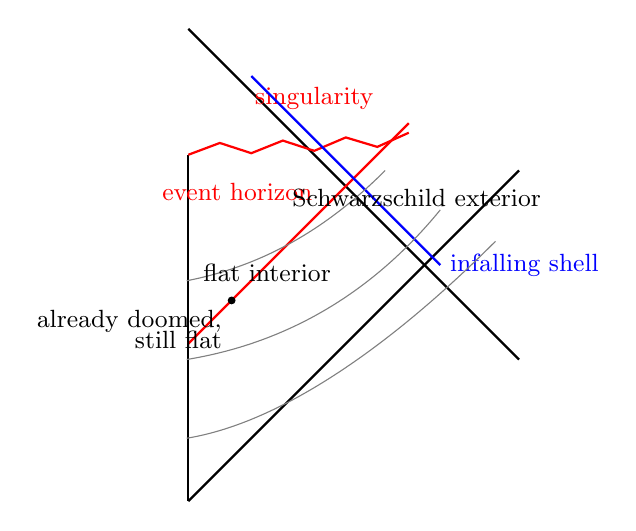
\begin{tikzpicture}[scale=1.0]
\draw[thick] (0,-3.0) -- (0,1.4);
\draw[thick] (0,3.0) -- (4.2,-1.2);
\draw[thick] (0,-3.0) -- (4.2,1.2);

\draw[red,thick] (0.0,1.4) -- (0.4,1.55) -- (0.8,1.42) -- (1.2,1.58) -- (1.6,1.45) -- (2.0,1.62) -- (2.4,1.50) -- (2.8,1.68);
\node[red,above] at (1.6,1.85) {\small singularity};

\draw[thick,red] (0,-1.0) -- (2.8,1.8);
\node[red,above left] at (1.7,0.7) {\small event horizon};

\draw[thick,blue] (3.2,0.0) -- (0.8,2.4);
\node[blue,right] at (3.2,0.0) {\small infalling shell};

\draw[gray] (-0.02,-2.2) .. controls (1.2,-2.0) and (2.6,-1.0) .. (3.9,0.3);
\draw[gray] (-0.02,-1.2) .. controls (1.2,-1.0) and (2.3,-0.4) .. (3.2,0.7);
\draw[gray] (-0.02,-0.2) .. controls (1.0,0.0) and (1.8,0.5) .. (2.5,1.2);

\filldraw (0.55,-0.45) circle (1.2pt);
\node[below left] at (0.55,-0.45) {\small already doomed,};
\node[below left] at (0.55,-0.72) {\small still flat};

\node at (1.0,-0.1) {\small flat interior};
\node at (2.9,0.85) {\small Schwarzschild exterior};
\end{tikzpicture}
\caption{A second transcript-backed reconstruction of the collapse diagram, now emphasizing the backward-traced event horizon. Part of the horizon lies in a region that is still locally flat and has not yet been reached by the shell.}
\end{figure}

This produces the striking effect on which the lecture dwells. Part of the horizon lies in a region that is still flat spacetime. The shell has not yet arrived there. An observer there may feel nothing special, may see no incoming shell in the backward light cone, and yet may already be doomed. The reason is not local and it is not mechanical. It is global and causal.

\subsection{Question \& Answer}

\paragraph{Question.} How can an observer already be doomed in flat spacetime, before the shell has reached them?

\paragraph{Answer.} Because the horizon is not a material membrane. It is the global boundary between escape and no escape. Inside the shell the geometry can still be flat, and crossing the shell may be the first locally noticeable encounter with matter or radiation. But the event horizon is defined by the complete future of the spacetime. If from a given event no future-directed causal curve reaches \(\mathscr I^+\), then that event lies inside the horizon even if locally nothing dramatic has happened yet.

The lecture repeatedly answers objections of the form ``before according to which time?'' by emphasizing that time is only a coordinate. An \emph{instant of time} really means a chosen spacelike slice. One may choose many such foliations, and the shell may be outside the horizon on some slice and inside it on another. The causal conclusion does not change. Different slicings change simultaneity, not the escape structure.

This is also where the distinction between the shell and the horizon becomes sharp. Crossing the shell can mean crossing actual matter or radiation. Crossing the horizon need not mean any local jolt at all. The shell may be locally detectable; the horizon need not be. That is why the lecture calls the horizon a little ghostly. It has causal significance without being a material surface.

One can phrase the same point in a more practical way. If the shell is incoming at the speed of light, an observer trapped inside the backward-traced horizon cannot get out of its way without exceeding the speed of light. The lecture turns this into an explicit example: even if the shell is still far away, perhaps millions of miles away, one may nevertheless be unable to outrun the growing trapped region. The diagram is the proof.

This also explains why mirror-rescue stories fail once one is sufficiently deep in the doomed region. If a reflecting structure had been placed early enough and far enough out, one could alter the causal history and prevent trapping. But once the relevant event lies behind the horizon, there is no longer enough causal time to send the structure to the needed location. A mirror placed inside the horizon is just another doomed object; it, the light, and the observer all end at the singularity.

Finally, the proper-time statement should be kept straight. From a generic horizon-crossing event to the singularity there is a finite proper time. Only the ideal corner where the singularity meets \(\mathscr I^+\) is infinitely far away, and trying to cling to that corner would require unbounded acceleration. It is not a physical escape route.

\section{Summary}

The lecture closes with a methodological lesson. Penrose diagrams do not preserve metric size, and they are not supposed to. They preserve the motion of light rays and, with it, the causal structure of spacetime. That is why they are so powerful.

For the Schwarzschild black hole, compactification turns the local Kruskal picture into a global causal picture. It shows the exterior, the doomed interior, the finite proper-time approach to the singularity, and the formal status of the extra quadrants. For the collapsing shell, it does more: it lets us build the spacetime by gluing flat interior to Schwarzschild exterior, and then identify the horizon as a global boundary rather than a locally detectable wall. The final moral is therefore exactly the one the lecture insists on: the physically important question is not how large a region looks on the page, but who can send a signal to whom, and who cannot escape.